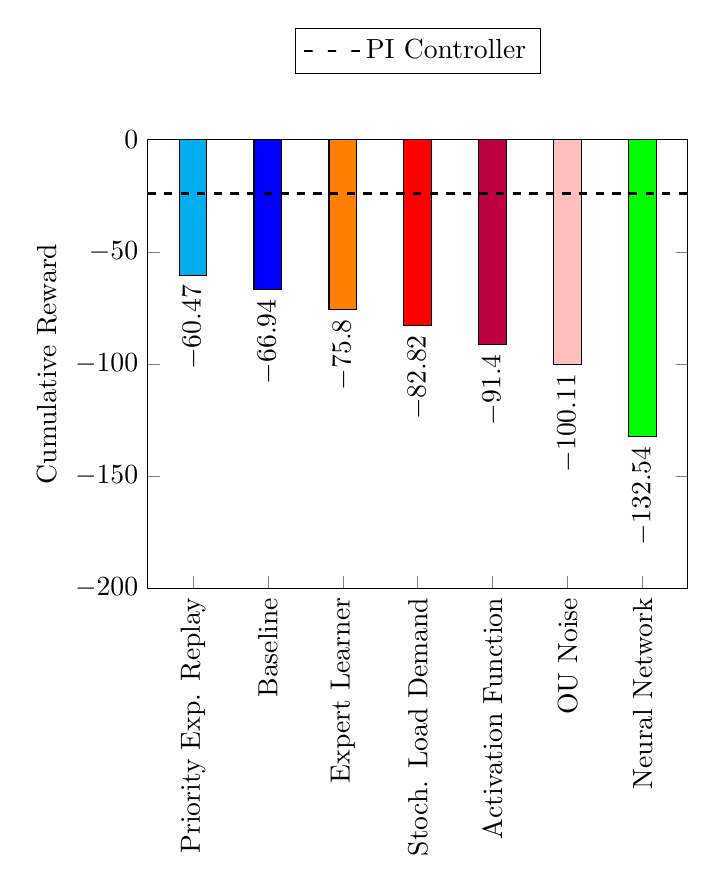
\begin{tikzpicture}
	\begin{axis}[
	    ylabel={Cumulative Reward},
	    symbolic x coords={Priority Exp. Replay,, Baseline,, Expert Learner,, Stoch. Load Demand,, Activation Function,, OU Noise,, Neural Network},
	    xtick = {Baseline, Neural Network, Activation Function, OU Noise, Priority Exp. Replay, Expert Learner, Stoch. Load Demand},
	    xticklabel style={rotate=90},
	    nodes near coords,
	    nodes near coords align={vertical},
	    every node near coord/.append style={rotate=90, anchor=east},
	    ymin=-200, ymax=0,
	    legend style={at={(0.5,1.25)},anchor=north}
	    ]
	\addplot [ybar, fill=blue] coordinates {(Baseline, -66.94)};
	\addplot [ybar, fill=green] coordinates {(Neural Network, -132.54)};
	\addplot [ybar, fill=purple] coordinates {(Activation Function, -91.40)};
	\addplot [ybar, fill=pink] coordinates {(OU Noise, -100.11)};
	\addplot [ybar, fill=cyan] coordinates {(Priority Exp. Replay, -60.47)};
	\addplot [ybar, fill=orange] coordinates {(Expert Learner, -75.80)};
	\addplot [ybar, fill=red] coordinates {(Stoch. Load Demand, -82.82)};
	%\legend{Baseline, Neural Network, Activation Function, OU Noise, Priority Experience Replay, Expert Learner, Stochastic Load Demand};
	\addplot[thick, black,dashed,sharp plot,nodes near coords={},update limits=false,shorten >=-10mm,shorten <=-10mm] 
			coordinates {(Priority Exp. Replay,-23.99) (Neural Network,-23.99)};
	\addlegendentry{PI Controller};
	\end{axis}
\end{tikzpicture}